\chapter{Elektroniczny system pomiarów}
Układ pomiarowy składa się z wcześniej przedstawionych urządzeń:

\begin{enumerate}
\setlength{\itemsep}{2pt} 
\setlength{\parskip}{2pt} 
\setlength{\parsep}{2pt}
\item mikrokomputer BeagleBone Black
\item czujnik ciśnienia i temperatury BMP085
\item czujnik wilgotności i temperatury DHT-22
\end{enumerate}

Kolejnym krokiem przy tworzeniu systemu pomiarów warunków środowiskowych i meteorologicznych jest poprawne podłączenie czujników do mikrokomputera, aby móc zbierać dane. Wykorzystując tabelę PINów, zainstalowanych w mikrokomputerze BeagleBone Black, podpięto czujniki według poniższej instrukcji:

\textbf{Czujnik BMP085:}
\begin{itemize}
\setlength{\itemsep}{2pt} 
\setlength{\parskip}{2pt} 
\setlength{\parsep}{2pt}
\item GND należy podłączyć do pinu P9.1 BeagleBone'a
\item VCC do pinu P9.3
\item SCL do pinu P9.19
\item SDA do pinu P9.20
\end{itemize}

\textbf{Czujnik DHT-22:}
\begin{itemize}
\setlength{\itemsep}{2pt} 
\setlength{\parskip}{2pt} 
\setlength{\parsep}{2pt}
\item GND należy podłączyć do pinu P9.2 BeagleBone'a
\item VDD do pinu P9.8
\item DATA do pinu P8.26
\end{itemize}

\begin{figure}[h!]
\centering
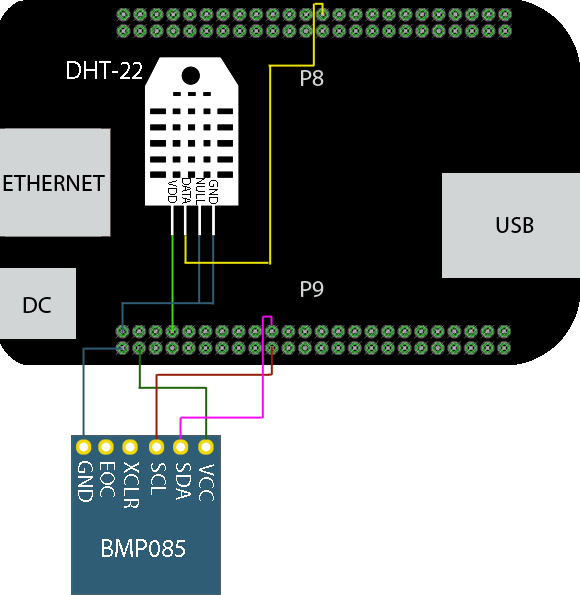
\includegraphics[scale=1.3]{uklad}
\caption{Zbudowany układ pomiarowy}
\label{fig:uklad}
\end{figure}

Sposób poprawnego podpięcia układu został również zamieszczony w formie rysunku (rys. \ref{fig:uklad}).

Cały układ pomiarowy został połączony ze sobą przy użyciu płytki stykowej. Jest to najlepsze rozwiązanie, jeżeli potrzebne jest tymczasowe rozwiązanie. Takie połączenia można dowolnie i w każdej chwili konfigurować, bez tworzenia nowej płytki drukowanej.

Docelowo planowane jest stworzenie płytki drukowanej w formie nakładki na BeagleBone'a, która idealnie będzie pasować do pinów wyprowadzonych z mikrokomputera.

Wadami tymczasowego rozwiązania wykorzysującego płytkę stykową jest możliwość zabrudzenia się otworów, co może spowodować wzrost oporu, a nawet brak łączności. Kolejną niedoskonałością jest łatwość przypadkowego rozpięcia układu, które często prowadzi do błędnych pomiarów.